% Options for packages loaded elsewhere
\PassOptionsToPackage{unicode}{hyperref}
\PassOptionsToPackage{hyphens}{url}
\documentclass[
]{book}
\usepackage{xcolor}
\usepackage{amsmath,amssymb}
\setcounter{secnumdepth}{5}
\usepackage{iftex}
\ifPDFTeX
  \usepackage[T1]{fontenc}
  \usepackage[utf8]{inputenc}
  \usepackage{textcomp} % provide euro and other symbols
\else % if luatex or xetex
  \usepackage{unicode-math} % this also loads fontspec
  \defaultfontfeatures{Scale=MatchLowercase}
  \defaultfontfeatures[\rmfamily]{Ligatures=TeX,Scale=1}
\fi
\usepackage{lmodern}
\ifPDFTeX\else
  % xetex/luatex font selection
\fi
% Use upquote if available, for straight quotes in verbatim environments
\IfFileExists{upquote.sty}{\usepackage{upquote}}{}
\IfFileExists{microtype.sty}{% use microtype if available
  \usepackage[]{microtype}
  \UseMicrotypeSet[protrusion]{basicmath} % disable protrusion for tt fonts
}{}
\makeatletter
\@ifundefined{KOMAClassName}{% if non-KOMA class
  \IfFileExists{parskip.sty}{%
    \usepackage{parskip}
  }{% else
    \setlength{\parindent}{0pt}
    \setlength{\parskip}{6pt plus 2pt minus 1pt}}
}{% if KOMA class
  \KOMAoptions{parskip=half}}
\makeatother
\usepackage{longtable,booktabs,array}
\newcounter{none} % for unnumbered tables
\usepackage{calc} % for calculating minipage widths
% Correct order of tables after \paragraph or \subparagraph
\usepackage{etoolbox}
\makeatletter
\patchcmd\longtable{\par}{\if@noskipsec\mbox{}\fi\par}{}{}
\makeatother
% Allow footnotes in longtable head/foot
\IfFileExists{footnotehyper.sty}{\usepackage{footnotehyper}}{\usepackage{footnote}}
\makesavenoteenv{longtable}
\usepackage{graphicx}
\makeatletter
\newsavebox\pandoc@box
\newcommand*\pandocbounded[1]{% scales image to fit in text height/width
  \sbox\pandoc@box{#1}%
  \Gscale@div\@tempa{\textheight}{\dimexpr\ht\pandoc@box+\dp\pandoc@box\relax}%
  \Gscale@div\@tempb{\linewidth}{\wd\pandoc@box}%
  \ifdim\@tempb\p@<\@tempa\p@\let\@tempa\@tempb\fi% select the smaller of both
  \ifdim\@tempa\p@<\p@\scalebox{\@tempa}{\usebox\pandoc@box}%
  \else\usebox{\pandoc@box}%
  \fi%
}
% Set default figure placement to htbp
\def\fps@figure{htbp}
\makeatother
\ifLuaTeX
  \usepackage{luacolor}
  \usepackage[soul]{lua-ul}
\else
  \usepackage{soul}
\fi
\setlength{\emergencystretch}{3em} % prevent overfull lines
\providecommand{\tightlist}{%
  \setlength{\itemsep}{0pt}\setlength{\parskip}{0pt}}
\usepackage[]{natbib}
\bibliographystyle{plainnat}
% ============================================================
% preamble.tex – for CS 598 Practical Statistical Learning
% This file is only used when rendering the PDF version
% ============================================================

\usepackage{microtype}
\microtypesetup{activate=false}   % optional – silences some warnings
\usepackage{silence}
\WarningFilter{mathtools}{For best results}
\WarningFilter{microtype}{Unable to apply patch}


% ----- Better tables -----
\usepackage{booktabs}          % Professional-looking tables (\toprule, \midrule, \bottomrule)

% ----- Math packages -----
\RequirePackage{mathtools}          % force early loading
\usepackage{amsmath}
\usepackage{amssymb}
\usepackage{amsfonts}
\usepackage{bm}
\usepackage{dsfont}



% Nice indicator function and blackboard bold
\usepackage{dsfont}            % \mathds{1} for indicator function
% \usepackage{bbm}             % alternative: \mathbbm{1}

% ----- Algorithms -----
\usepackage{algorithm}         % Floating algorithm environment
\usepackage{algpseudocode}     % Nice pseudocode commands (\Procedure, \State, \If, etc.)

% ----- Figures & graphics -----
\usepackage{graphicx}          % Including images
\usepackage{float}             % Allows [H] placement specifier for figures/tables
\usepackage{subcaption}        % Subfigures and subtables

% ----- Hyperlinks & cross-references -----
\usepackage{hyperref}
\hypersetup{
  colorlinks = true,
  linkcolor  = blue,           % internal links (figures, sections, equations)
  citecolor  = blue,           % citations
  urlcolor   = blue,           % external URLs
  bookmarks  = true
}

% ----- Lists & spacing -----
\usepackage{enumitem}          % Better control over itemize/enumerate
\usepackage{setspace}          % Optional: control line spacing if needed

% ----- Colors (useful for custom boxes or highlighting) -----
\usepackage{xcolor}

% ----- Page layout (optional – uncomment if you want to change margins) -----
% \usepackage{geometry}
% \geometry{margin=1in}

% ============================================================
% Optional custom commands (examples – add more as you need)
% ============================================================


% Example: shortcut for independent and identically distributed
\newcommand{\iid}{\overset{\text{iid}}{\sim}}

% Example: argmin / argmax
\DeclareMathOperator*{\argmin}{arg\,min}
\DeclareMathOperator*{\argmax}{arg\,max}

% Example: indicator function shortcut


\newcommand{\ind}{\mathds{1}}
\usepackage{bookmark}
\IfFileExists{xurl.sty}{\usepackage{xurl}}{} % add URL line breaks if available
\urlstyle{same}
\hypersetup{
  pdftitle={CS 598 Practical Statistical Learning},
  pdfauthor={Alexandra Chronopoulou},
  hidelinks,
  pdfcreator={LaTeX via pandoc}}

\title{CS 598 Practical Statistical Learning}
\author{Alexandra Chronopoulou}
\date{2026-08-19}

\begin{document}
\maketitle

{
\setcounter{tocdepth}{1}
\tableofcontents
}
\chapter*{Course Information}\label{course-information}
\addcontentsline{toc}{chapter}{Course Information}

Course Description

This course provides an introduction to modern techniques for statistical analysis of complex and massive data. Examples of these include model selection for regression, classification, nonparametric models such as splines and kernel models, regularization, dimension reduction, and clustering analysis. Applications are discussed as well as computation and theoretical foundations.

~

Course Prerequisites

Knowledge of basic multivariate calculus, statistical inference, and linear algebra. You should be comfortable with the following concepts: probability distribution functions, expectations, conditional distributions, likelihood functions, random samples, estimators, and linear regression models.

~

Course Learning Outcomes

By the end of the course, you will be able to:

\begin{itemize}
\tightlist
\item
  Use a broad range of methods and techniques in machine learning.
\item
  Have a deeper understanding of major algorithms and techniques in machine learning.
\item
  Build analytics pipelines for regression problems.
\item
  Build analytics pipelines for classification problems.
\item
  Build analytics pipelines for recommendation problems.
\end{itemize}

~

Textbook and Readings

There is no required textbook for this course.

Recommended resources for a statistical approach to machine learning are:

\begin{itemize}
\tightlist
\item
  \emph{An Introduction to Statistical Learning with Applications in R} (basic)
\item
  \emph{An Introduction to Statistical Learning with Applications in Python} (basic)
\item
  \emph{The Elements of Statistical Learning: Data Mining, Inference, and Prediction} (more advanced)
\end{itemize}

You may also want to view the \href{https://www.youtube.com/playlist?list=PL5-da3qGB5IDMEgF2WXqfCG5nfztd8r_n}{Data School YouTube videos} associated with the first book as an additional resource.

~

The detailed syllabus for the course can be found on Coursera.

\chapter{Introduction to Statistical Learning}\label{introduction-to-statistical-learning}

\textbf{Statistical Learning} is a field at the intersection of statistics, computer science, and data science that focuses on developing and understanding models that can \emph{learn} from data. While statistics has long dealt with model building, validation, and prediction, the dramatic growth in the volume, complexity, and dimensionality of data has strained many classical techniques. The introduction of sophisticated algorithms, data-management tools, and optimization methods from computer science has enabled more powerful approaches suited to modern data regimes.

In the supervised setting, learning from data typically means that, given an outcome (quantitative or categorical) and a (usually large) set of features, we construct a \textbf{prediction model} (also called a \emph{learner}) that can accurately forecast the outcome for new, previously unseen observations.

~

We can separate statistical learning problems in \ul{\emph{two types}}:

\begin{itemize}
\tightlist
\item
  \textbf{Supervised Learning}: when an outcome variable is present to guide the learning process. The two primary examples are:

  \begin{itemize}
  \tightlist
  \item
    \emph{Regression}: Response is quantitative (continuous or discrete numeric).
  \item
    \emph{Classification}: Response is categorical (binary or multi-class).
  \end{itemize}
\item
  \textbf{Unsupervised Learning}:when an outcome variable is not present to guide the learning process. The goal is to discover latent structure or patterns in the data (e.g., clustering, association rules, hidden Markov models, etc.).
\end{itemize}

\section{Examples of Statistical Learning Problems}\label{examples-of-statistical-learning-problems}

Birthweight Data: A Regression Example

This dataset comes from a study whose goal is to predict the birth weight of a newborn from a collection of baby and parental characteristics (gestation length, length, head circumference, mother's and father's height, mother's weight, parental smoking status, etc.). The study focuses particularly on babies born prematurely (before 40 weeks of gestation).

The scatterplot matrix below shows the pairwise relationships among the variables in the dataset:

\begin{center}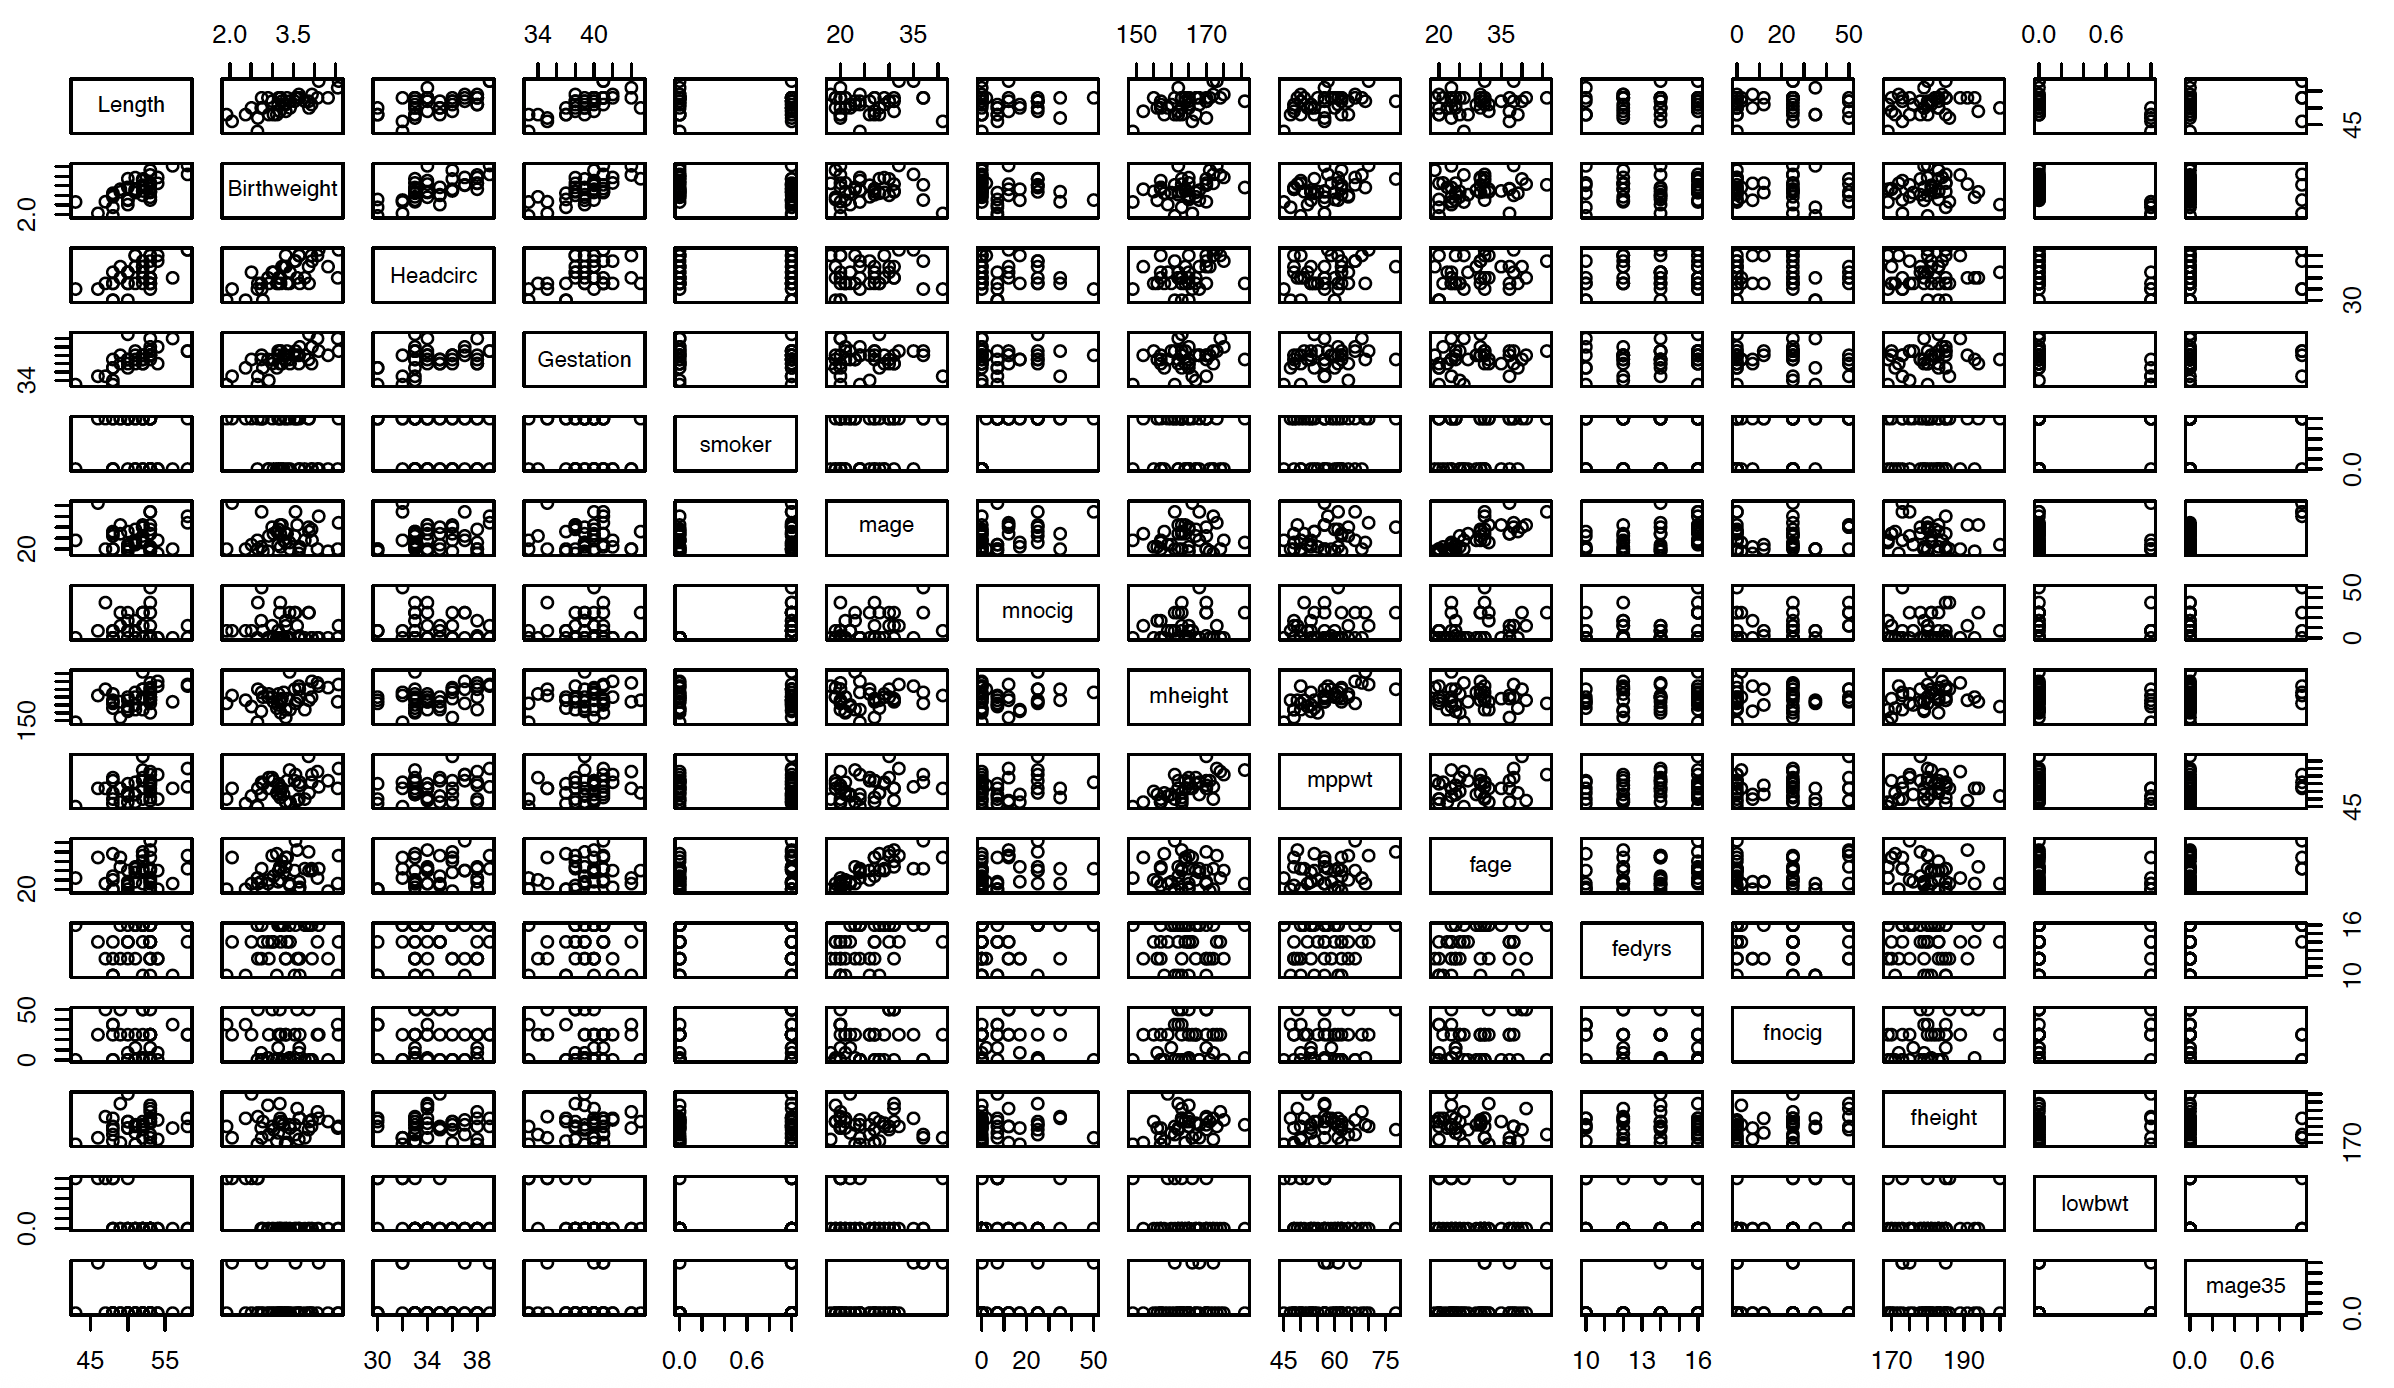
\includegraphics[width=1\linewidth]{images/week1/birthpairs} \end{center}

Note that three of the predictors (\texttt{smoker}, \texttt{lowbwt}, and \texttt{mage35}) are categorical.

This is a classic example of a supervised regression problem and a natural setting in which a multiple linear regression (MLR) model can be considered. If the MLR model fits well and the key assumptions are reasonably satisfied, it can provide useful predictions of birth weight for new observations.

~

Trees and Shrubs Data: A Binary Classification Example

In this problem, the goal is to predict whether a woody plant common in the Black Forest region of southwestern Germany is a tree or a shrub (Lederer). A sample of the data is shown below:

\begin{tabular}{l|r|r|r|r|l}
\hline
Name & Height & Diameter & GrowthRate & Longevity & Type\\
\hline
Silver Fir & 55.0 & 1.50 & 0.5 & 500 & Tree\\
\hline
European Beech & 40.0 & 1.00 & 0.5 & 200 & Tree\\
\hline
Common Hazel & 5.0 & 0.10 & 0.5 & 70 & Shrub\\
\hline
Red Raspberry & 1.5 & 0.01 & 0.4 & 10 & Shrub\\
\hline
European Spruce & 50.0 & 1.20 & 0.5 & 600 & Tree\\
\hline
\end{tabular}

This is a binary classification problem in which we want to use a set of characteristics to predict the class label (tree or shrub).

~

Handwritten Digits: A Multiclass Classification Example

This is a classic multiclass classification problem in which the goal is to predict the handwritten digit \((0, \ldots, 9)\) appearing on a postal envelope, based on a 16 \(\times\) 16 eight-bit grayscale image (ESL). The practical challenge is to keep the error rate sufficiently low so that mail is not misdirected.

\begin{center}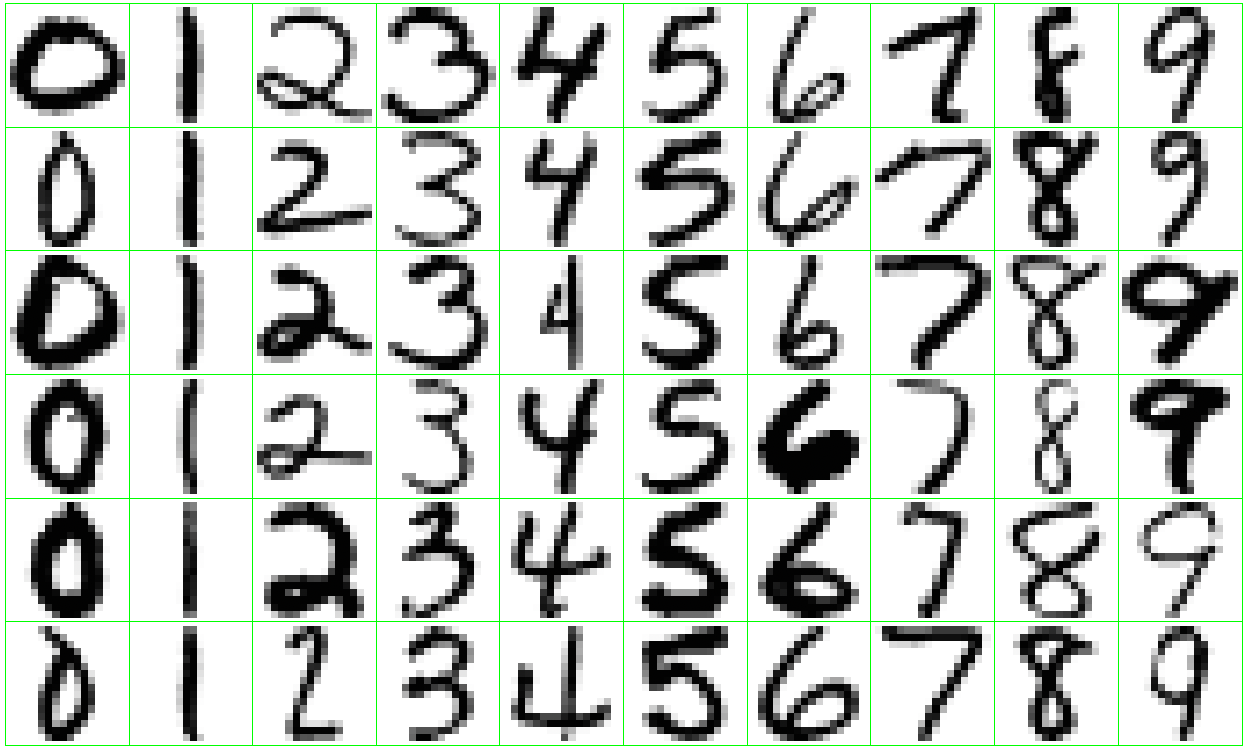
\includegraphics[width=0.75\linewidth]{images/week1/SLEx_digits} \end{center}

~

Proteomics Data: A Clustering Example

Proteomics is the large-scale study of proteins. Data of this type are typically generated through laboratory processes such as protein purification or mass spectrometry (a technique that measures the mass-to-charge ratio of ions).

The figure below shows an expression matrix for 437 proteins, of which only 101 are of primary interest (Romanova et al.). A common challenge with such data is the large amount of missing values (shown as grey pixels). The goal is to cluster the proteins into coherent groups for further biological analysis.

\begin{center}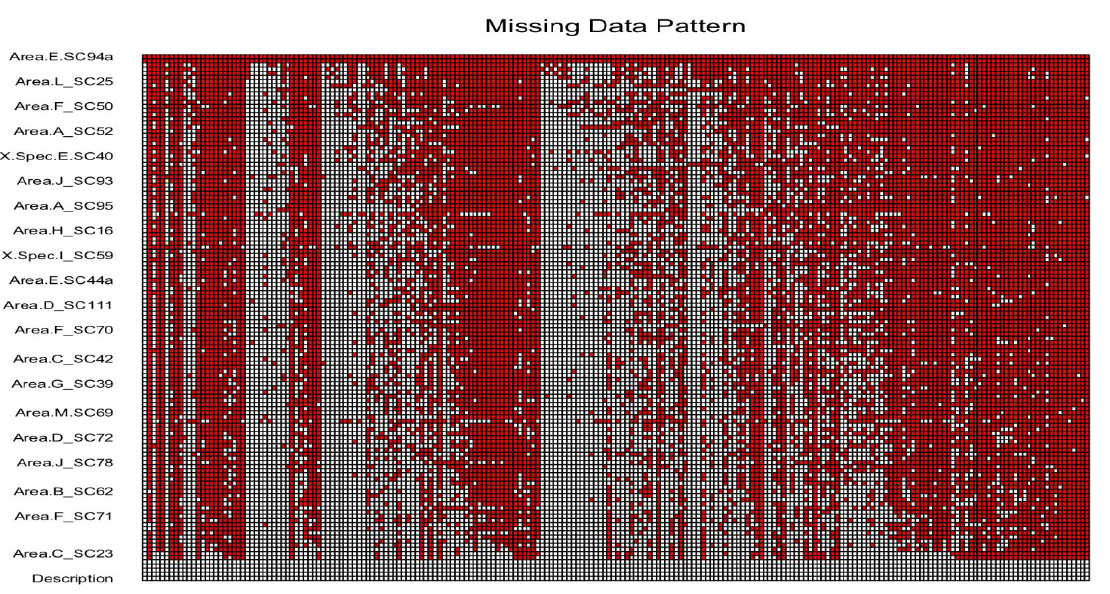
\includegraphics[width=0.85\linewidth]{images/week1/chemistry} \end{center}

~

These examples illustrate the variety of problems that arise in statistical learning. The birthweight data is a typical supervised regression problem in which we aim to predict a quantitative outcome. The trees-and-shrubs data is a binary classification task, while the handwritten-digit data is a multiclass classification problem. Finally, the proteomics data is an unsupervised learning example whose goal is to uncover latent structure through clustering. Together they show how statistical learning methods can be applied across different types of outcomes and data structures, whether the aim is \emph{prediction} or the \emph{discovery of patterns}.

\section{Supervised Learning Framework}\label{supervised-learning-framework}

In this class, our main focus is \textbf{supervised learning}. This means that we observe \textbf{target} (\emph{outcome}, \emph{response}) variable \(Y\) that we wish to predict using a set of \emph{features} (\emph{predictors}), \(X\). We assume that the relationship between the response \(Y\) and the features is given by a function \(f\) that is known up to a parameter vector \(w\):
\[\mathbf{Y} = f(\mathbf{X}, w) + varepsilon \]
When \(f\) is fully known except for the value of \(w\) (for example when \(f\) is linear), then learning problem reduces to \textbf{estimating} \(w\). To do so, we collect a \textbf{training sample} \(\bigl\{\mathbf{x}_i, \mathbf{y}_i  \bigr\}_{i=1}^{n}\) and minimize an \textbf{objective} function\_with respect to \(w\):
\[F(w) = \sum_{i=1}^{n} loss \Bigl(y_i,\, f \bigl(\mathbf{x}_i, w \bigr) \Bigr)\]
The \textbf{loss} function measures the discrepancy between the model prediction \(f(\mathbf{x}_i, w)\) and the observed outcome \(\mathbf{y}_i\). The choice of loss is made by the practitioner; the most common examples are:

\begin{itemize}
\item
  \textbf{Squared Error Loss}
  \[\text{loss} = \Bigl[ y_i - f\bigl(x_i; w \bigr)\Bigr]^2\]
\item
  \textbf{Absolute Error Loss}
  \[\text{loss} = \Bigl| y_i - f\bigl(x_i; w \bigr)\Bigr|\]
\item
  \textbf{Log Loss} (binary classification)
  \[\text{loss} = -y_i \log f(x_i; w) - (1-y_i)\log\bigl(1 - f(x_i; w)\bigr) \]
\item
  \textbf{0-1 Loss}
  \[\text{loss} =\mathbf{1}_{\{y_i \neq \hat{y}_i\}}
  \quad\text{where}\quad
  \hat{y}_i = f(x_i; w) \]
\end{itemize}

Depending on the chosen loss, the minimizer of \(F(w)\) may or may not admit a closed-form expression. When a closed form is unavailable we resort to numerical optimization algorithms. In many cases gradient-based methods (in particular gradient descent and its variants) can be used to obtain a good solution.

~

\section{Why Statistical Learning is Challenging}\label{why-statistical-learning-is-challenging}

In the framework of the previous section we reduced the learning problem to the estimation of a parameter vector \(w\), under the assumption that the true function \(f\) is known up to this parameter. In practice, however, we rarely know the exact form of \(f\). We must therefore \emph{approximate} it by some function \(\hat{f}\). This approximation introduces an \emph{additional source of error}.

Moreover, the objective function we minimize is computed on a \emph{training} sample. While this quantifies how well the model fits the observed data, the real goal of statistical learning is good performance on \textbf{new}, \textbf{unseen} data. In other words, we aim to minimize the \textbf{test error} (also called generalization error), not the training error.

\emph{Statistical learning is therefore challenging for several reasons}:

\begin{itemize}
\item
  The training error typically underestimates the test/generalization error.
\item
  A model may perform well on the training data yet poorly on future data because of overfitting.
  The number of parameters required to approximate \(f\) can be large---sometimes larger than the number of available observations.
\item
  As the number of model parameters grows, the test error often increases substantially.
\end{itemize}

~

Two simple illustrations make these points concrete:

\begin{enumerate}
\def\labelenumi{\arabic{enumi}.}
\item
  \textbf{Classification: 1-Nearest Neighbour}\\
  The one-nearest-neighbour classifier achieves zero training error (it predicts every training point perfectly) but typically performs poorly on test data. An instructive demonstration of how increasing dimensionality affects the performance of linear classifiers can be found \href{https://www.visiondummy.com/2014/04/curse-dimensionality-affect-classification/}{here}.
\item
  \textbf{Regression: the \(p\) versus \(n\) problem}\\
  Consider the linear model
  \[
  \mathbf{y}_{n\times 1} = \mathbf{X}_{n\times p}\mathbf{w}_{p\times 1} + \varepsilon,
  \]
  where \(\mathbf{y}\) is the response vector, \(\mathbf{X}\) is the design matrix with \(p\) predictors, and \(\mathbf{w}\) contains the coefficients to be estimated.

  \begin{itemize}
  \tightlist
  \item
    When \(p < n\) we have more equations than parameters; classical regression methods usually work well.
  \item
    When \(p = n\) we have exactly as many equations as parameters and can achieve a perfect fit on the training data.
  \item
    When \(p > n\) we have fewer equations than parameters. In this high-dimensional regime classical methods break down and specialized techniques are required.
  \end{itemize}
\end{enumerate}

~

In summary, statistical learning is challenging because we must approximate an unknown function \(f\), control the gap between training and test error, and often operate in regimes where the number of parameters is large relative to the sample size. Successfully addressing these issues is essential for building models that generalize well to new data.

\section{Bias-Variance Trade-Off}\label{bias-variance-trade-off}

We have already noted that \emph{two sources of error} affect the quality of our predictions. In statistical learning we must balance:

\begin{itemize}
\tightlist
\item
  \textbf{Bias}: the systematic difference between the average of our estimated function \(\hat{f}\) and the true underlying function \(f\). High bias typically leads to under-fitting and an inaccurate model.
\item
  \textbf{Variance}: the amount by which \(\hat{f}\) would change if we estimated it using a different training sample. High variance typically leads to over-fitting and an unreliable model.
\end{itemize}

A helpful analogy is to think of the learning problem as a \textbf{target} whose \emph{center represents the true model}.

\begin{center}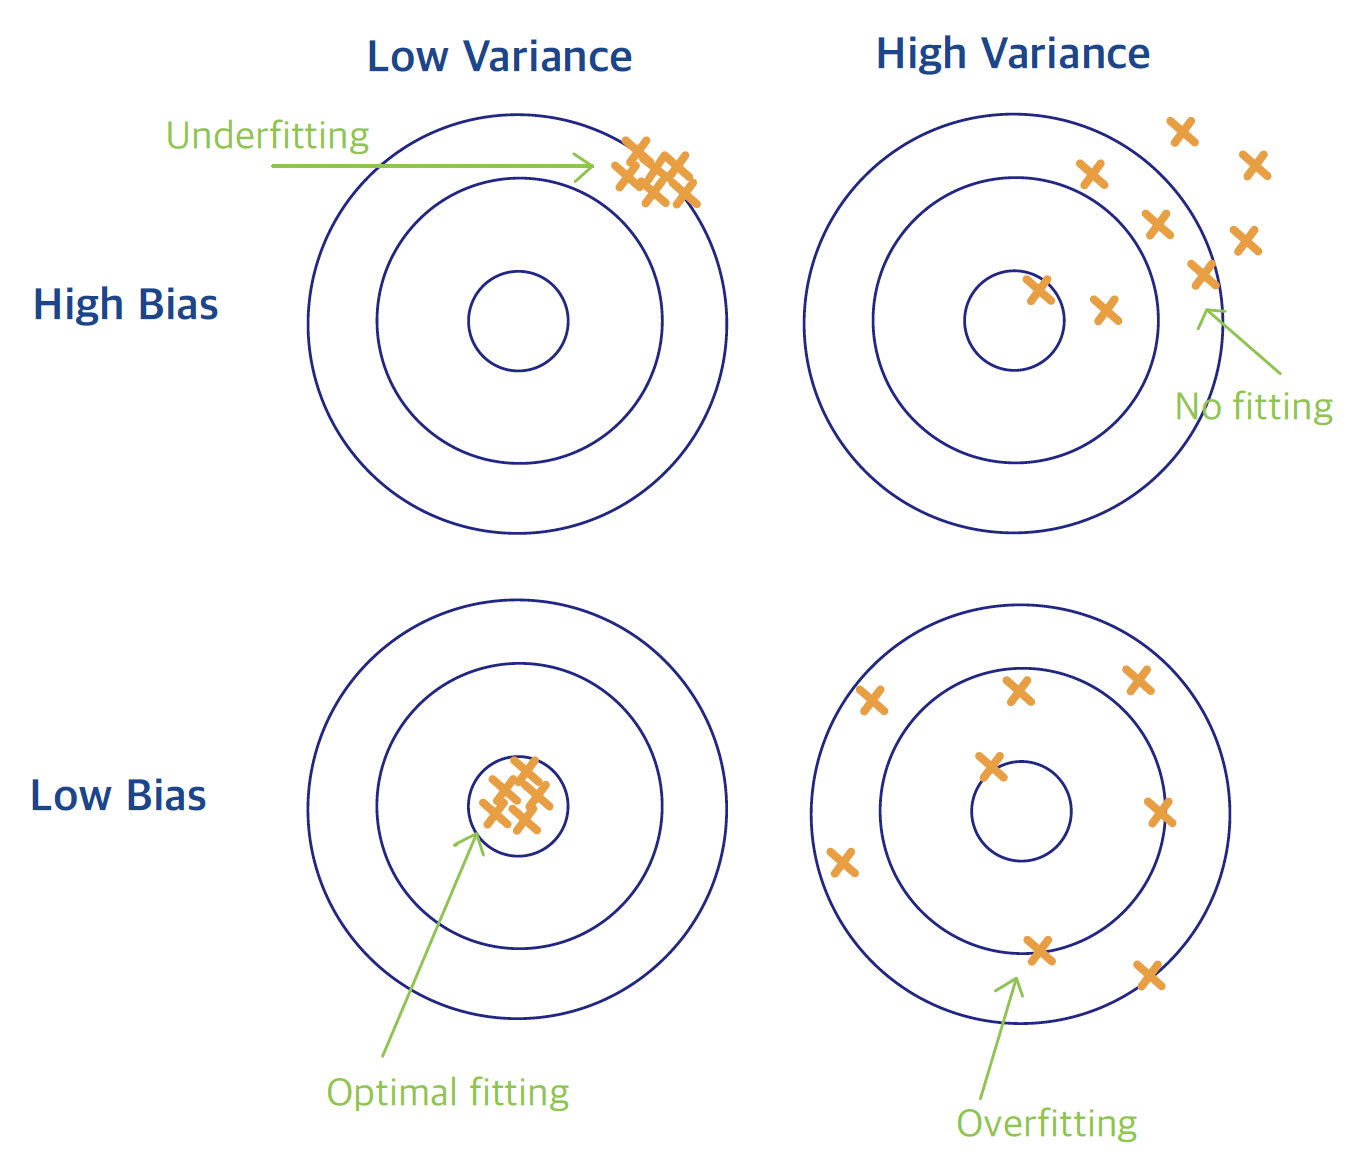
\includegraphics[width=0.6\linewidth]{images/week1/tradeoff1} \end{center}

How close the fitted values lie to the center is measured by bias. If the points systematically miss the center, the model is a poor approximation of \(f\). Increasing the sample size will not correct a large bias.
The spread of the fitted values around their average is measured by variance. When the points are tightly clustered the variance is low; when they are widely scattered the variance is high.

Ideally we would like to reduce both bias and variance simultaneously. In practice this is not possible, so we must trade one against the other. Remembering that our ultimate goal is to minimize the generalization (test) error, not the training error, we observe the following typical behavior:

\begin{center}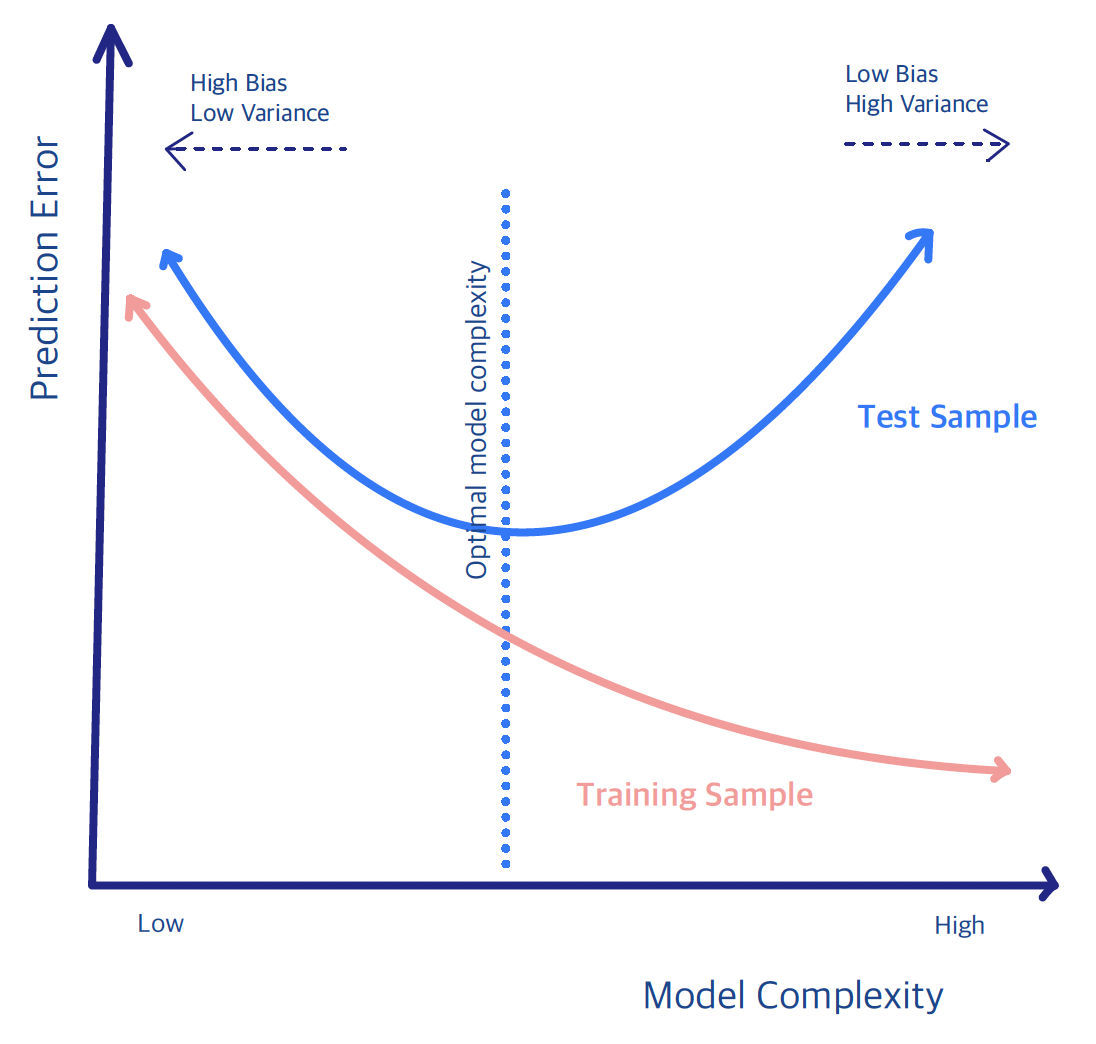
\includegraphics[width=0.5\linewidth]{images/week1/traintest2} \end{center}

\begin{itemize}
\item
  When the model is highly complex (many parameters), the training error tends to decrease. However, the model often over-fits the training data and therefore exhibits high variance on new data, resulting in poor generalization.
\item
  When the model is very simple (few parameters), it tends to under-fit the data. This produces large bias and, again, poor generalization performance.
\end{itemize}

~

In this class we will discuss:

\begin{enumerate}
\def\labelenumi{(\roman{enumi})}
\item
  flexible modeling techniques that help reduce bias, and
\item
  practical strategies for achieving a good bias-variance trade-off.
\end{enumerate}

~

Two important approaches that we will study in detail are:

\begin{itemize}
\item
  \textbf{Regularization}: constrain the parameters to a lower-dimensional space that is determined adaptively by the data.
\item
  \textbf{Ensemble}: average many low-bias, high-variance models; the averaging step reduces variance while largely preserving the low bias.
\end{itemize}

\section{\texorpdfstring{Two Toy Examples: \(k\)-NN vs.~Linear Regression}{Two Toy Examples: k-NN vs.~Linear Regression}}\label{two-toy-examples-k-nn-vs.-linear-regression}

Before we conclude this introductory chapter, we examine two simple supervised learning methods:

\begin{enumerate}
\def\labelenumi{(\roman{enumi})}
\tightlist
\item
  \(k\)-Nearest Neighbors (\(k\)-NN)\\
\item
  Linear regression
\end{enumerate}

We will compare their behavior on simple examples and use them to illustrate the bias-variance trade-off.

~

\subsection{\texorpdfstring{\(k\)-Nearest Neighbors}{k-Nearest Neighbors}}\label{k-nearest-neighbors}

In the \textbf{\(k\)-nearest neighbors} (\(k\)-NN) method we predict the response at a point \(\mathbf{x}\) by using the \(k\) training observations that are closest to \(\mathbf{x}\). The \(k\)-NN fit is

\[\hat{\mathbf{y}}(\mathbf{x}) = \frac{1}{k} \sum_{x_i \in N_k(\mathbf{x})} y_i\]
where \(N_k(\mathbf{x})\) denotes the neighborhood of \(\mathbf{x}\) consisting of the \(k\) nearest training points.

\begin{itemize}
\tightlist
\item
  In \textbf{regression}, \(\hat{y}(\mathbf{x})\) is a local average of the neighboring responses.\\
\item
  In \textbf{classification}, \(\hat{y}(\mathbf{x})\) is the majority class (or the class probability) within the neighborhood.
\end{itemize}

Two practical challenges that arise are choosing the neighborhood size \(k\) and choosing the distance metric that defines the neighborhood.

The value of \(k\) directly controls model complexity, which is roughly proportional to \(n/k\).

\begin{itemize}
\tightlist
\item
  When \(k=1\) the prediction at each training point \(x_i\) is exactly \(y_i\), yielding zero training error.\\
\item
  When \(k=n\) every neighborhood contains the entire training sample, so the prediction is constant for all \(\mathbf{x}\).
\end{itemize}

The ``default'' metric is Euclidean distance

\[d\bigl( \mathbf{x}, \tilde{\mathbf{x}} \bigr) = \sum_{j=1}^{p} w_j \bigl( x_j - \tilde{x}_j \bigr)^2,\]
where the weights \(w_j\) may be learned from the data.

~

\subsection{Linear Regression}\label{linear-regression}

Given an input vector \(\mathbf{x}^\top = (x_1,\dots,x_p)\), we approximate the response by a linear function

\[f(\mathbf{x}) \approx \beta_0 + \sum_{j=1}^{p} x_j \beta_j\]

The coefficients \(\beta_j\) are estimated by ordinary least squares (OLS), i.e., by minimizing the residual sum of squares (\emph{objective function})

\[\min_{\beta_0, \ldots, \beta_p} \sum_{i=1}^{n} \Bigl( y_i - \beta_0 - x_{i1}\beta_1 - \ldots - x_{ip} \beta_p \Bigr)^2\]

Under standard conditions the solution has a closed form, and the fitted value at the \(i\)-th observation is

\[\hat{y}_i = \hat{y}(x_i) = x_i^T \hat{\beta}\]

We postpone the algebraic details until Week 2.

\subsubsection*{Linear Regression in a Classification Setting}\label{linear-regression-in-a-classification-setting}
\addcontentsline{toc}{subsubsection}{Linear Regression in a Classification Setting}

Linear regression can also be applied to binary classification problems in which \(Y\in\{0,1\}\). One simply predicts \texttt{class\ 1} when the fitted value \(\hat{f}(\mathbf{x})\) exceeds 0.5 and \texttt{class\ 0} otherwise.

This approach has well-known drawbacks: the squared-error loss is not a natural measure for binary outcomes, and a linear function can produce fitted values outside the interval \([0,1]\). For these reasons logistic regression is the preferred linear method for classification. It models the log-odds

\[\log \frac{p(\mathbf{x})}{1-p(\mathbf{x}) } \approx \beta_0 + \sum_{j=1}^{p} x_j \beta_j\]

We will return to logistic regression in Week 8.

~

\subsection{A Simulated (Binary) Classification Example}\label{a-simulated-binary-classification-example}

Consider a response variable \(G\) that takes two values (0 = BLUE or 1 = ORANGE). We generate 200 observations (100 in each class) and compare linear regression and \(k\)-nearest neighbors \textbf{as classifiers}.

The code used to produce the simulation and all figures is available in R and Python.

\subsubsection*{Linear Regression Classifier}\label{linear-regression-classifier}
\addcontentsline{toc}{subsubsection}{Linear Regression Classifier}

We first fit a linear regression model, treating the binary response as if it were continuous. The continuous fitted values \(\hat{Y}\) are then converted to class predictions \(\hat{G}\) by the simple rule
\[\hat{G} = \begin{cases}
& Blue, \text{ if } \hat{Y} > 0.5\\
& Orange, \text{ otherwise } \\
\end{cases} \]

Because the problem is two-dimensional, the decision boundary is a \emph{straight line}.

\begin{center}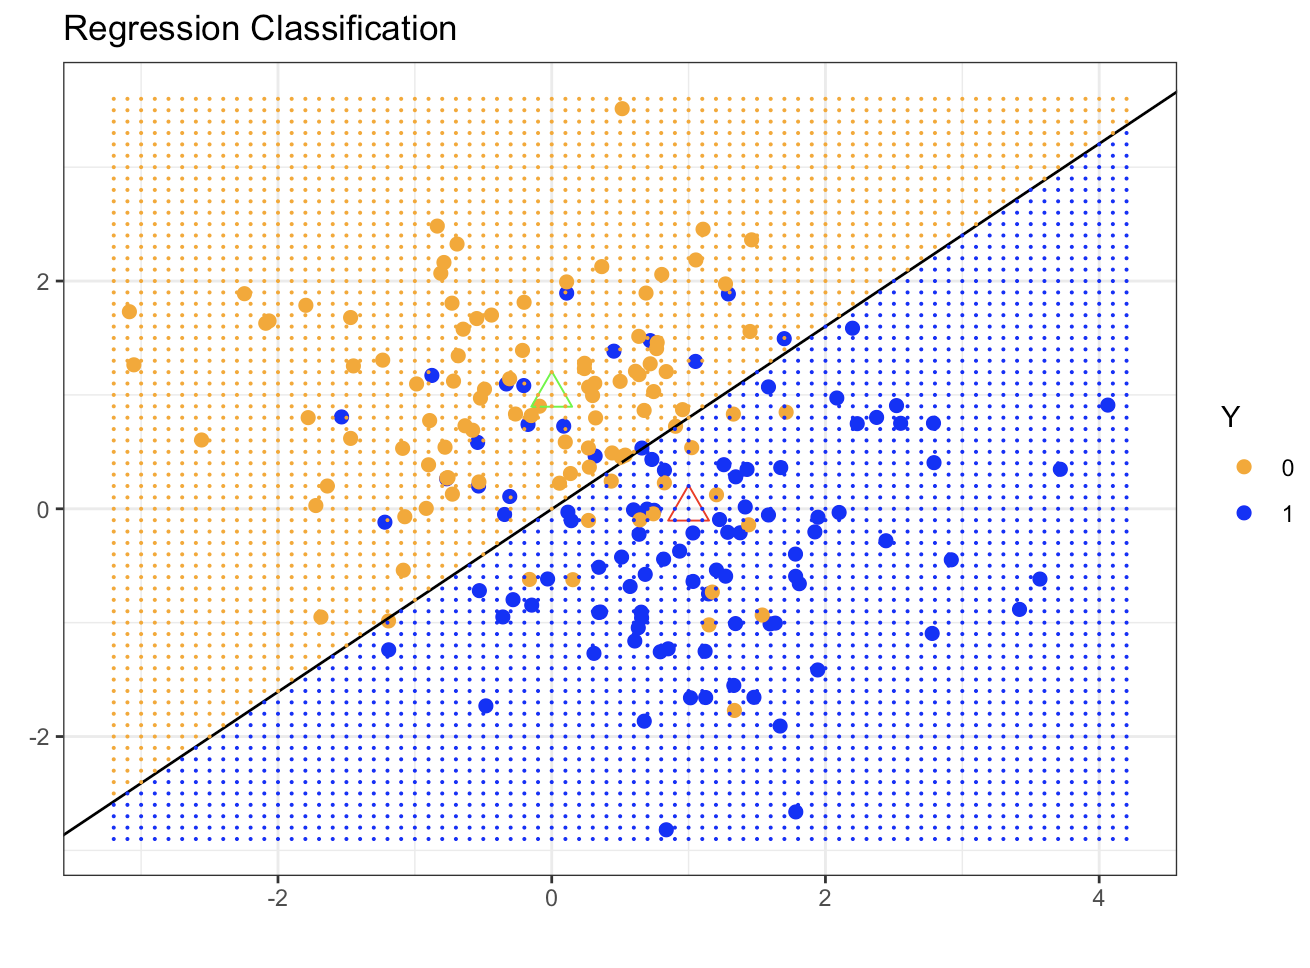
\includegraphics[width=0.7\linewidth]{images/week1/regclass} \end{center}

The fitted boundary (black line in the figure below) is the set of points satisfying \(\mathbf{x}^\top\hat{\beta} = 0.5\). In the simulation the true blue region lies above this line and the orange region below it. Many points on both sides of the boundary are nevertheless misclassified. The linear decision boundary is smooth but rigid; it cannot adapt to local structure in the data.

\subsubsection*{\texorpdfstring{\(k\)-Nearest-Neighbor Classifier}{k-Nearest-Neighbor Classifier}}\label{k-nearest-neighbor-classifier}
\addcontentsline{toc}{subsubsection}{\(k\)-Nearest-Neighbor Classifier}

We now apply \(k\)-nearest neighbors to the same data. Using \(k=15\), \(\hat{Y}(\mathbf{x})\) is the proportion of blue observations among the 15 nearest neighbors of \(\mathbf{x}\). Class labels are again assigned by the 0.5 threshold:

\[\hat{G} = \begin{cases}
& Blue, \text{ if } \hat{Y} > 0.5\\
& Orange,\text{ otherwise } \\
\end{cases} \]
(The prediction is therefore a majority vote among the 15 neighbors.)

\begin{center}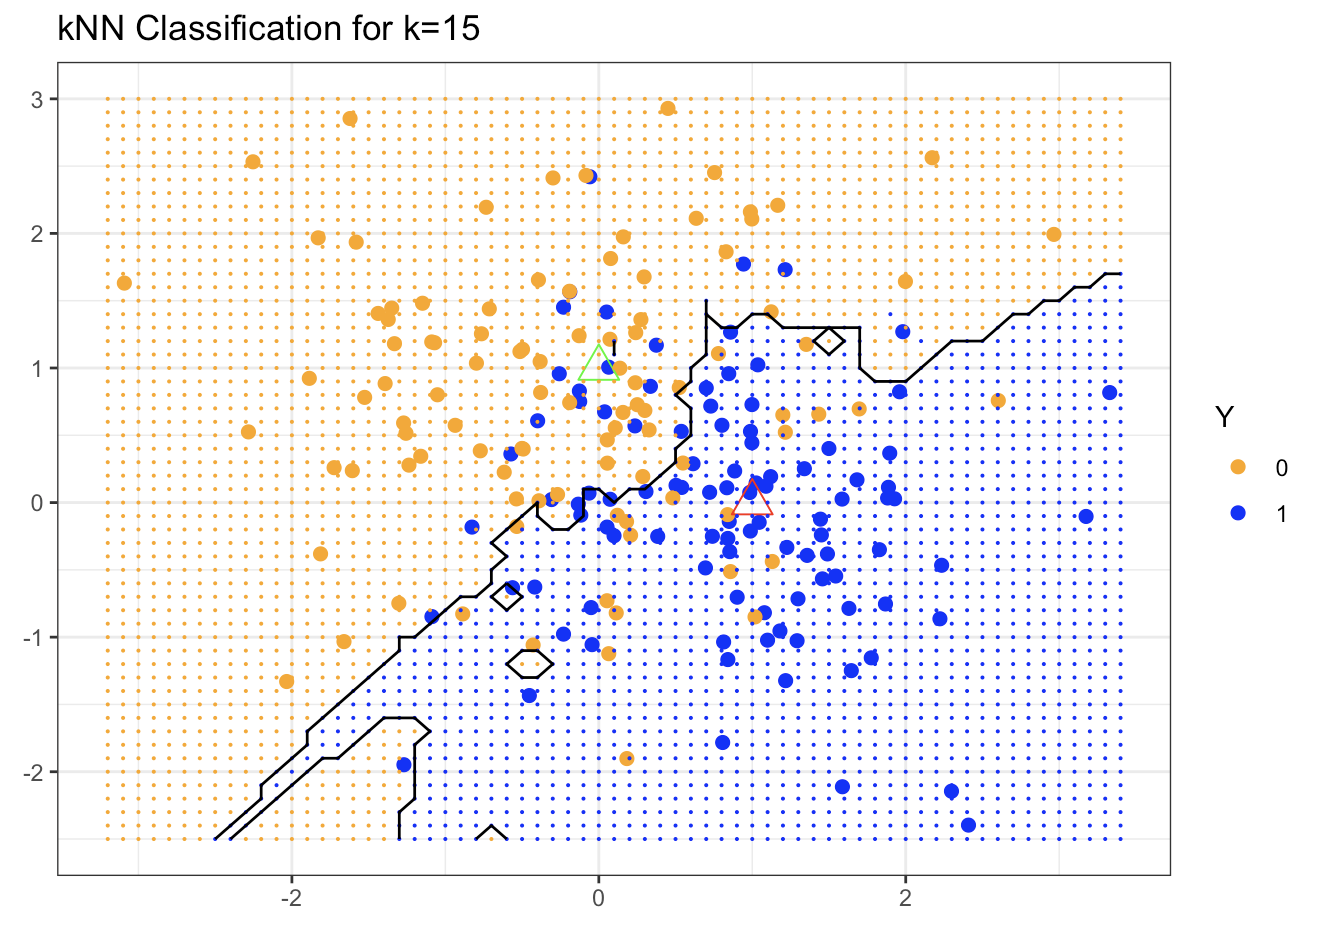
\includegraphics[width=0.7\linewidth]{images/week1/kNN15} \end{center}

The resulting decision boundary is far more irregular and follows local clusters of blue and orange points. Consequently the number of misclassifications on the training data is smaller than with linear regression.
If we take the extreme case \(k=1\), each point is classified by its single nearest neighbor:

\begin{center}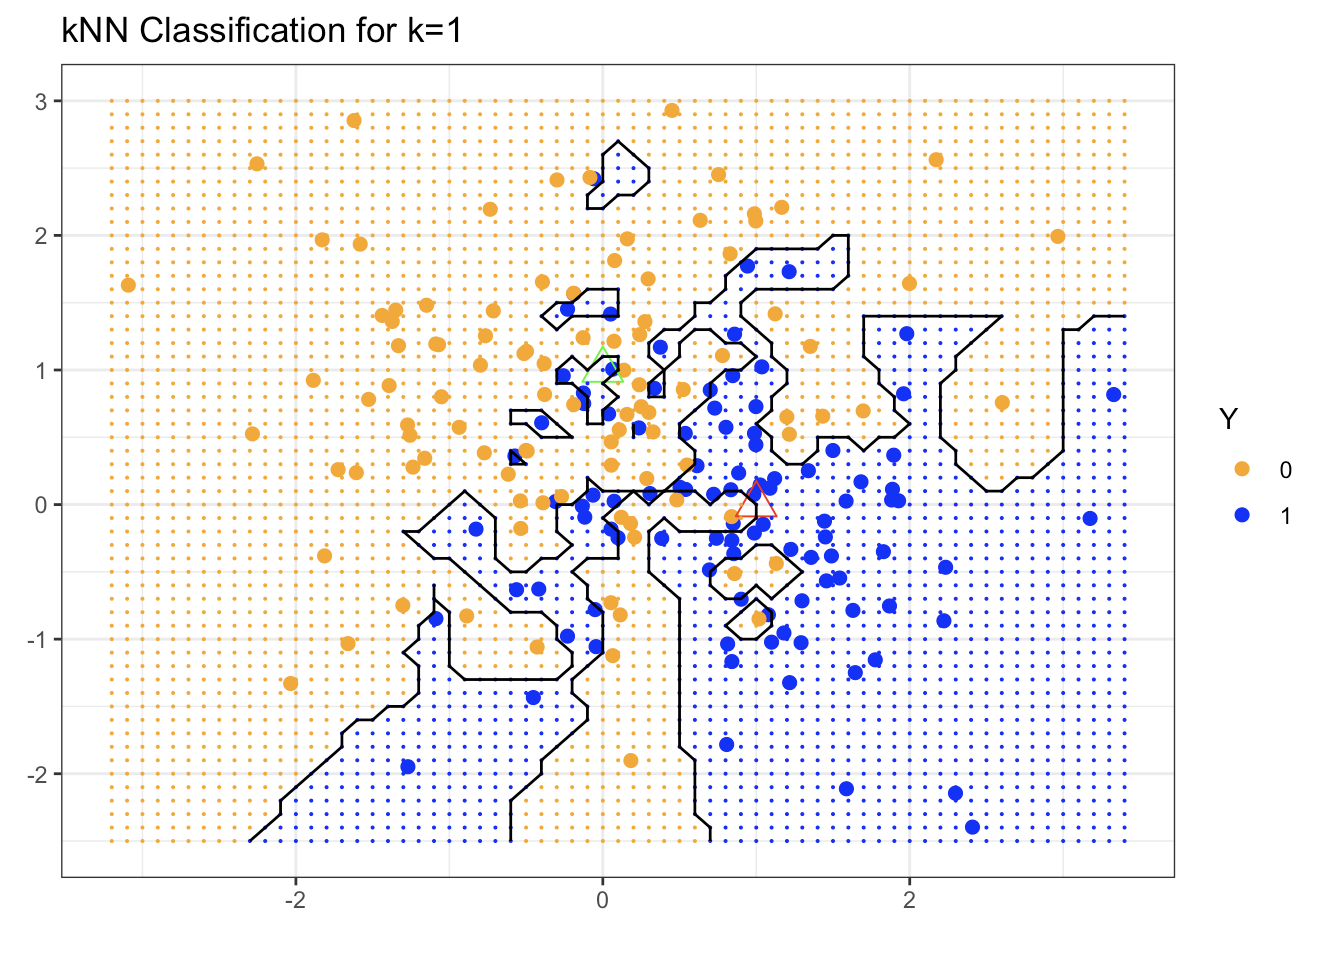
\includegraphics[width=0.7\linewidth]{images/week1/kNN1} \end{center}

The boundary becomes extremely rough and the training misclassification rate drops nearly to zero. Whether this is desirable, however, can be judged only by examining the \emph{generalization error}.

\subsubsection*{Training versus Test Error}\label{training-versus-test-error}
\addcontentsline{toc}{subsubsection}{Training versus Test Error}

Up to this point we have evaluated both methods on the same data that were used to fit them. A method such as 1-NN therefore appears to have zero error. Fair comparison requires an independent test set. The figure below shows misclassification error on a test set of 10,000 observations as a function of model degrees of freedom. Several \(k\)-NN fits (varying \(k\)) are compared with the linear regression fit.

\begin{center}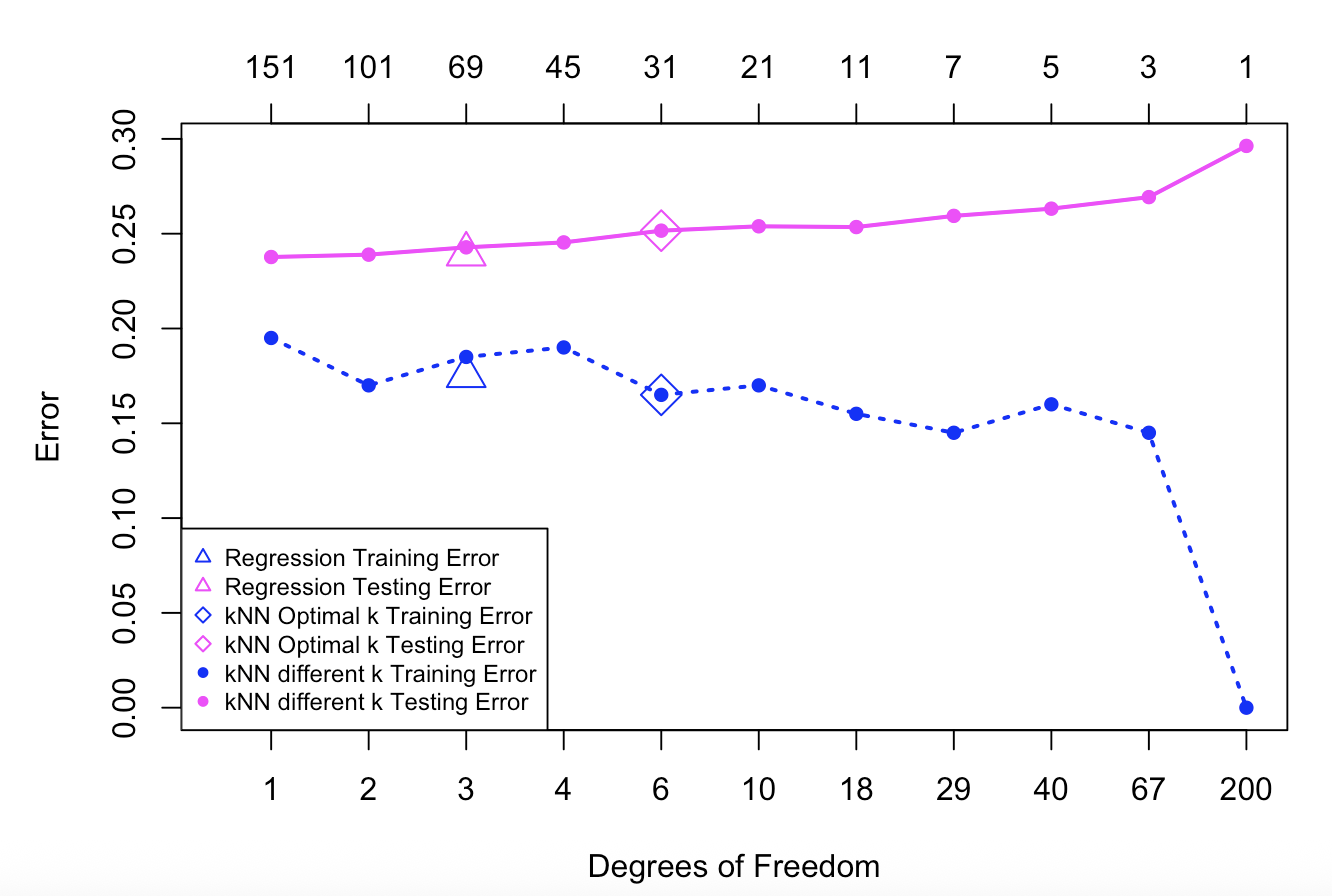
\includegraphics[width=0.7\linewidth]{images/week1/traintesterror} \end{center}

The magenta curve is the test error and the blue curve is the training error of \(k\)-NN. A 5-fold cross-validation procedure selected the optimal \(k\) (marked by a diamond). Linear regression results appear as the magenta and blue triangles at 3 degrees of freedom (the dimension of the fitted linear model).
Linear regression has only a few parameters and therefore relatively low variance, but the linearity assumption is restrictive for this problem and produces high bias.

In contrast, \(k\)-NN makes almost no assumption about the shape of the decision boundary (apart from a mild local-smoothness condition). This flexibility yields low bias but high variance; the extreme case \(k=1\) corresponds to roughly \(n\) parameters and severely overfits. It can be shown that \(k\)-NN is consistent when \(k,n\to\infty\) with \(k/n\to 0\). The price of that consistency is the high variance that appears when the effective number of parameters becomes large.

\bibliography{book.bib,packages.bib}

\end{document}
